\documentclass[american]{beamer}
\usepackage[T1]{fontenc}
\usepackage[utf8]{inputenc}
\setcounter{secnumdepth}{3}
\setcounter{tocdepth}{3}
\usepackage{amssymb}
\usepackage{graphicx}
\usepackage{babel}
\usepackage{amsmath}

\usetheme{Szeged}
\usecolortheme{beaver}


\title{A model of random walk with varying transition probabilities}
\institute[FNSPE CTU]{\inst{1} Faculty of Nuclear Sciences and Physical Engineering, CTU Prague \and
    \inst{2} Institute of Information Theory and Automation, CAS CR Prague}
%\date{16.9.2019}
\author[Tomáš~Kouřim]{Tomáš~Kouřim \inst{1} \and Petr Volf \inst{2}}
\newcommand{\nologo}{\setbeamertemplate{logo}{}} % command to set the logo to nothing
\setbeamertemplate{itemize item}[circle]
\setbeamertemplate{itemize subitem}[square]
\setbeamercovered{transparent}
%\logo{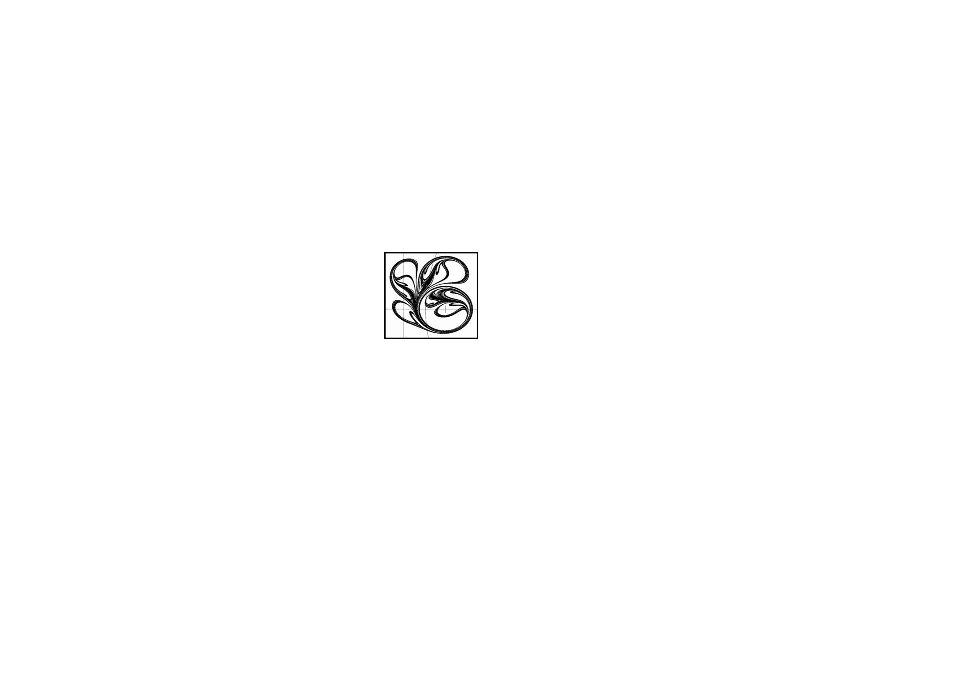
\includegraphics[height=1.3cm]{../CMSIM_Logo.pdf}}

\begin{document}
    \maketitle

    \begin{frame}{Outline}
        \begin{enumerate}
            \item<1-> {\Large{}Motivation}\bigskip{}
            \item<2-> {\Large{}Model description}\bigskip{}
            \item<3-> {\Large{}Model application}
        \end{enumerate}
    \end{frame}

    \begin{frame}{Random walk}
        \begin{definition}
            A man starts from a point $O$ and walks $l$ yards in a straight line;
            he then turns through any angle whatever and walks another $l$
            yards in a second straight line.
            He repeats this process $n$ times.
            I require the probability that after these $n$ stretches he is at
            a distance between $r$ and $r+\delta r$ from his starting point, $O$.

            {\footnotesize{}\medskip{}\emph{[Karl Pearson: The problem of the random walk.(1905)]}}

            \vspace{10mm}
            \begin{itemize}
                \item[]<2-> \large{Where is the \emph{drunken sailor}?}
            \end{itemize}
        \end{definition}
    \end{frame}

    \begin{frame}{Motivation}
        \begin{itemize}
            \item Failure of a machine
            \begin{itemize}
                \item repair after failure
                \item preventive maintenance
            \end{itemize}
            \item<2-> Occurrence of a disease
            \begin{itemize}
                \item cure of the disease
                \item prevention (i.e. lifestyle change)
            \end{itemize}
            \item<3-> Development of sports match
            \begin{itemize}
                \item goal scored, point achieved
                \item period won
            \end{itemize}
        \end{itemize}
    \end{frame}

    \begin{frame}{Random walk with varying probabilities}
        \begin{itemize}
            \item Random walk with memory
            \item Memory coefficient $\lambda\in(0,\,1)$ affecting the transition probabilities
            \item First step of the walk $X_{1}$ depends on an initial transition probability $p_{0}$
            \item Further steps depend on a transition probability $p_{t}$ evolving as
            \onslide<2->\begin{flalign*}
                            X_{t-1} & =1\rightarrow p_{t}=\lambda p_{t-1} &
                            X_{t-1} & =-1\rightarrow p_{t}=1-\lambda(1-p_{t-1}) &
            \end{flalign*}
            \vspace{-5mm}
            \begin{itemize}
                \item[-->]<3-> ``Success punished''
            \end{itemize}
            \onslide<4->\begin{flalign*}
                            X_{t-1}&=1\rightarrow p_{t}=1-\lambda(1-p_{t-1})&
                            X_{t-1}&=-1\rightarrow p_{t}=\lambda p_{t-1}&
            \end{flalign*}
            \vspace{-5mm}
            \begin{itemize}
                \item[-->]<5-> ``Success rewarded''
            \end{itemize}
        \end{itemize}
    \end{frame}

    \begin{frame}{Example - RW development}
        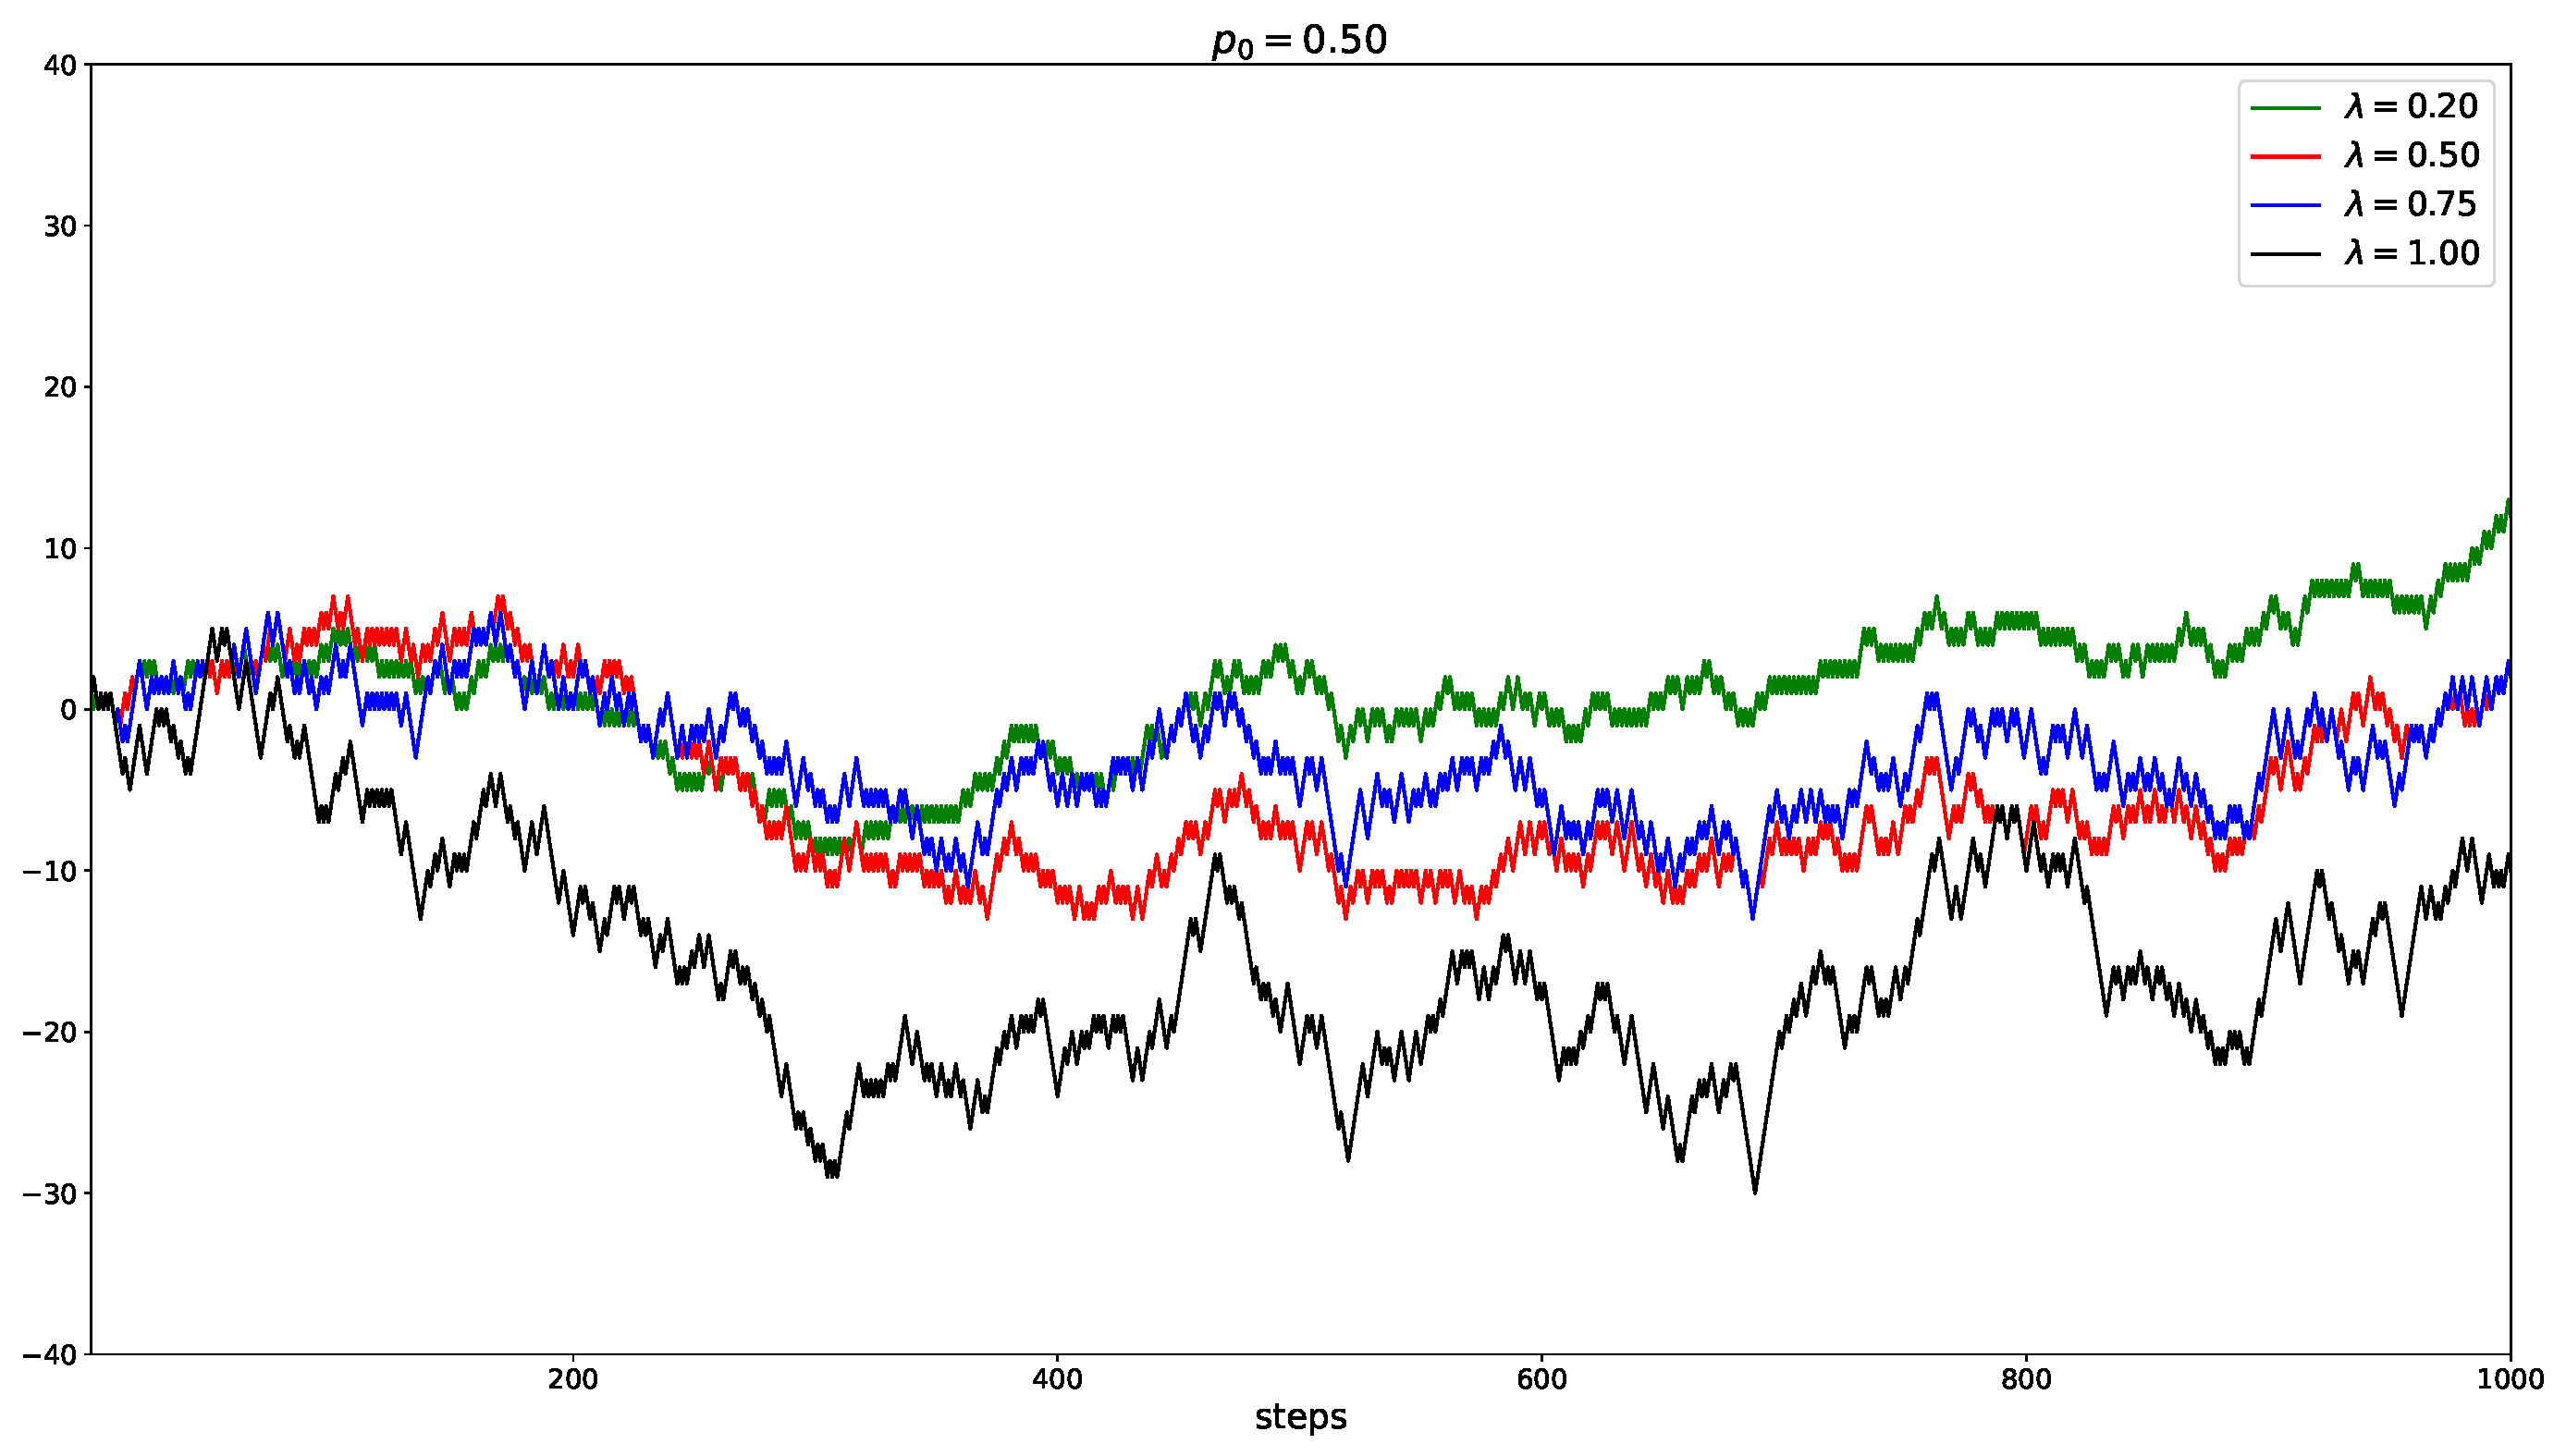
\includegraphics[width=1\textwidth]{../../simulations/single_walk_1000_steps_type_success_punished}
    \end{frame}

    \begin{frame}{Example - RW development}
        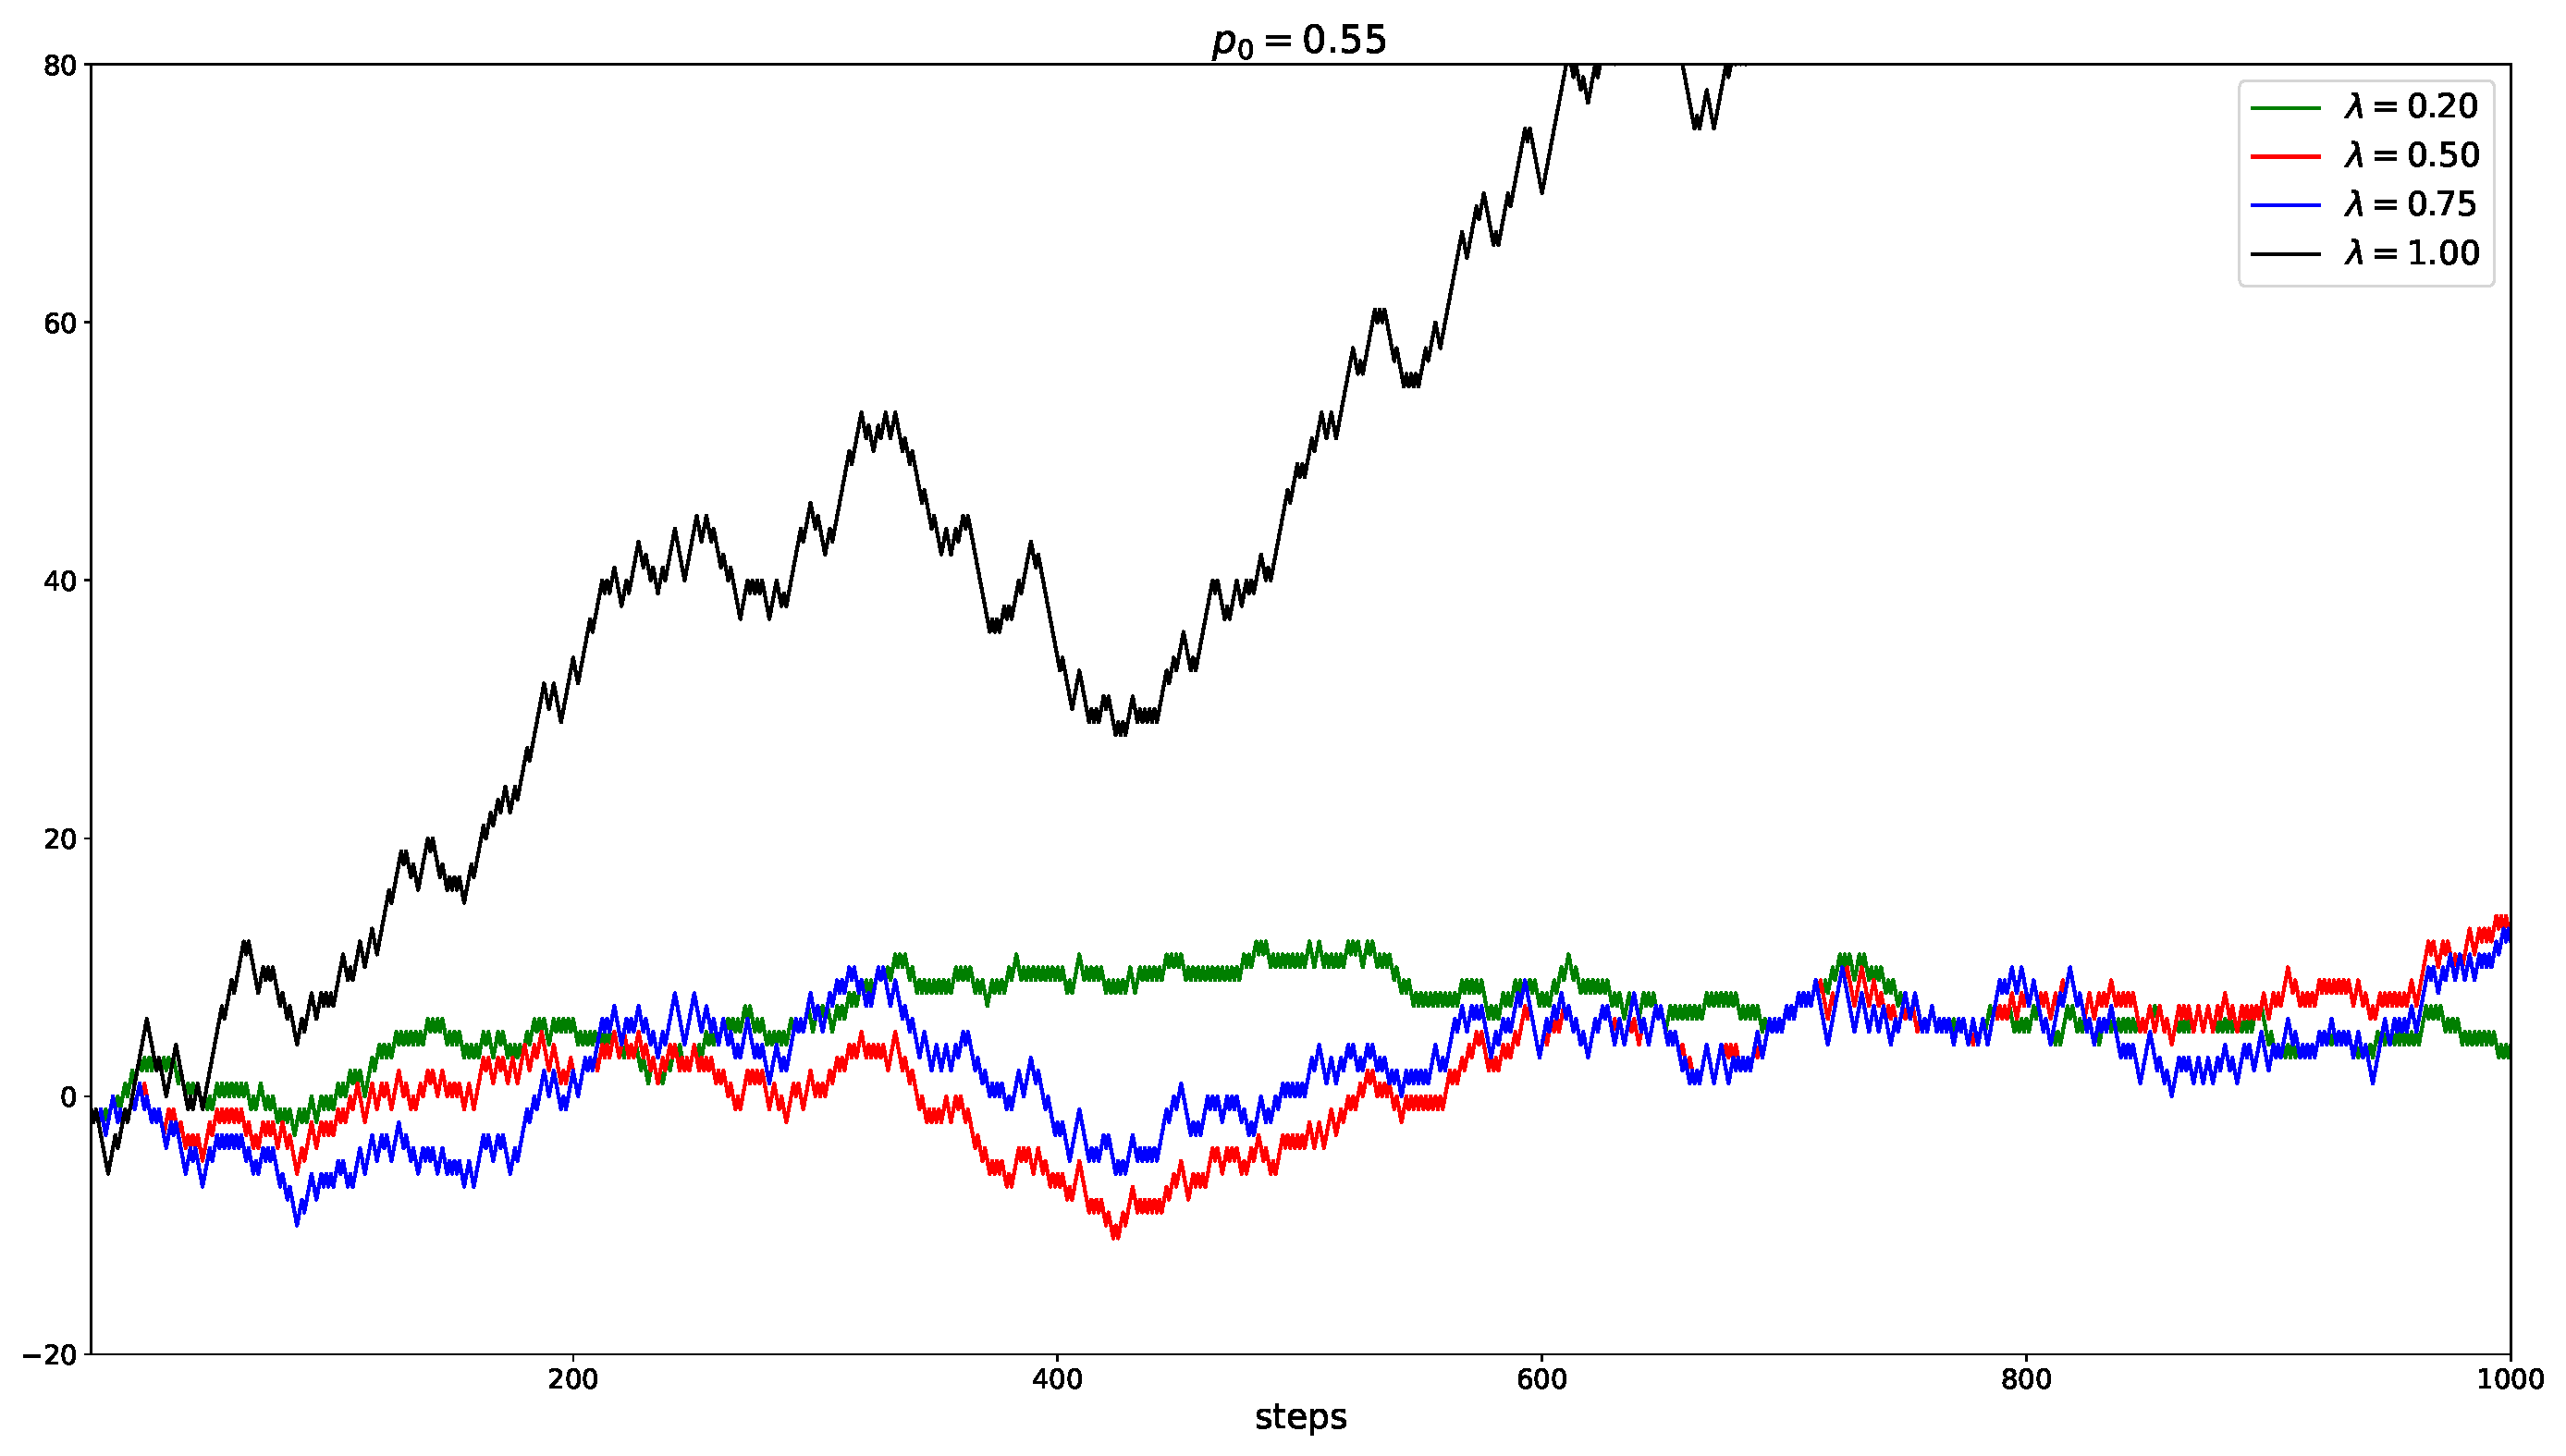
\includegraphics[width=1\textwidth]{../../simulations/single_walk_1000_steps_type_success_punished_p0_0.55}
    \end{frame}

    \begin{frame}{Walk steps properties}

        \begin{flalign*}
            EX_{t} & =(2\lambda-1)^{t-1}(2p_{0}-1)&
        \end{flalign*}
        \vspace{-5mm}
        \begin{flalign*}
            \lim_{t\to+\infty}EX_{t}&=0&
        \end{flalign*}
        \onslide<2->
        \begin{flalign*}
            Var\,X_{t}&=1-(2\lambda-1)^{2(t-1)}(2p_{0}-1)^{2}&
        \end{flalign*}
        \vspace{-5mm}
        \begin{flalign*}
            \lim_{t\to+\infty}Var\,X_{t}&=1&
        \end{flalign*}

    \end{frame}

    \begin{frame}{Example - RW steps}
        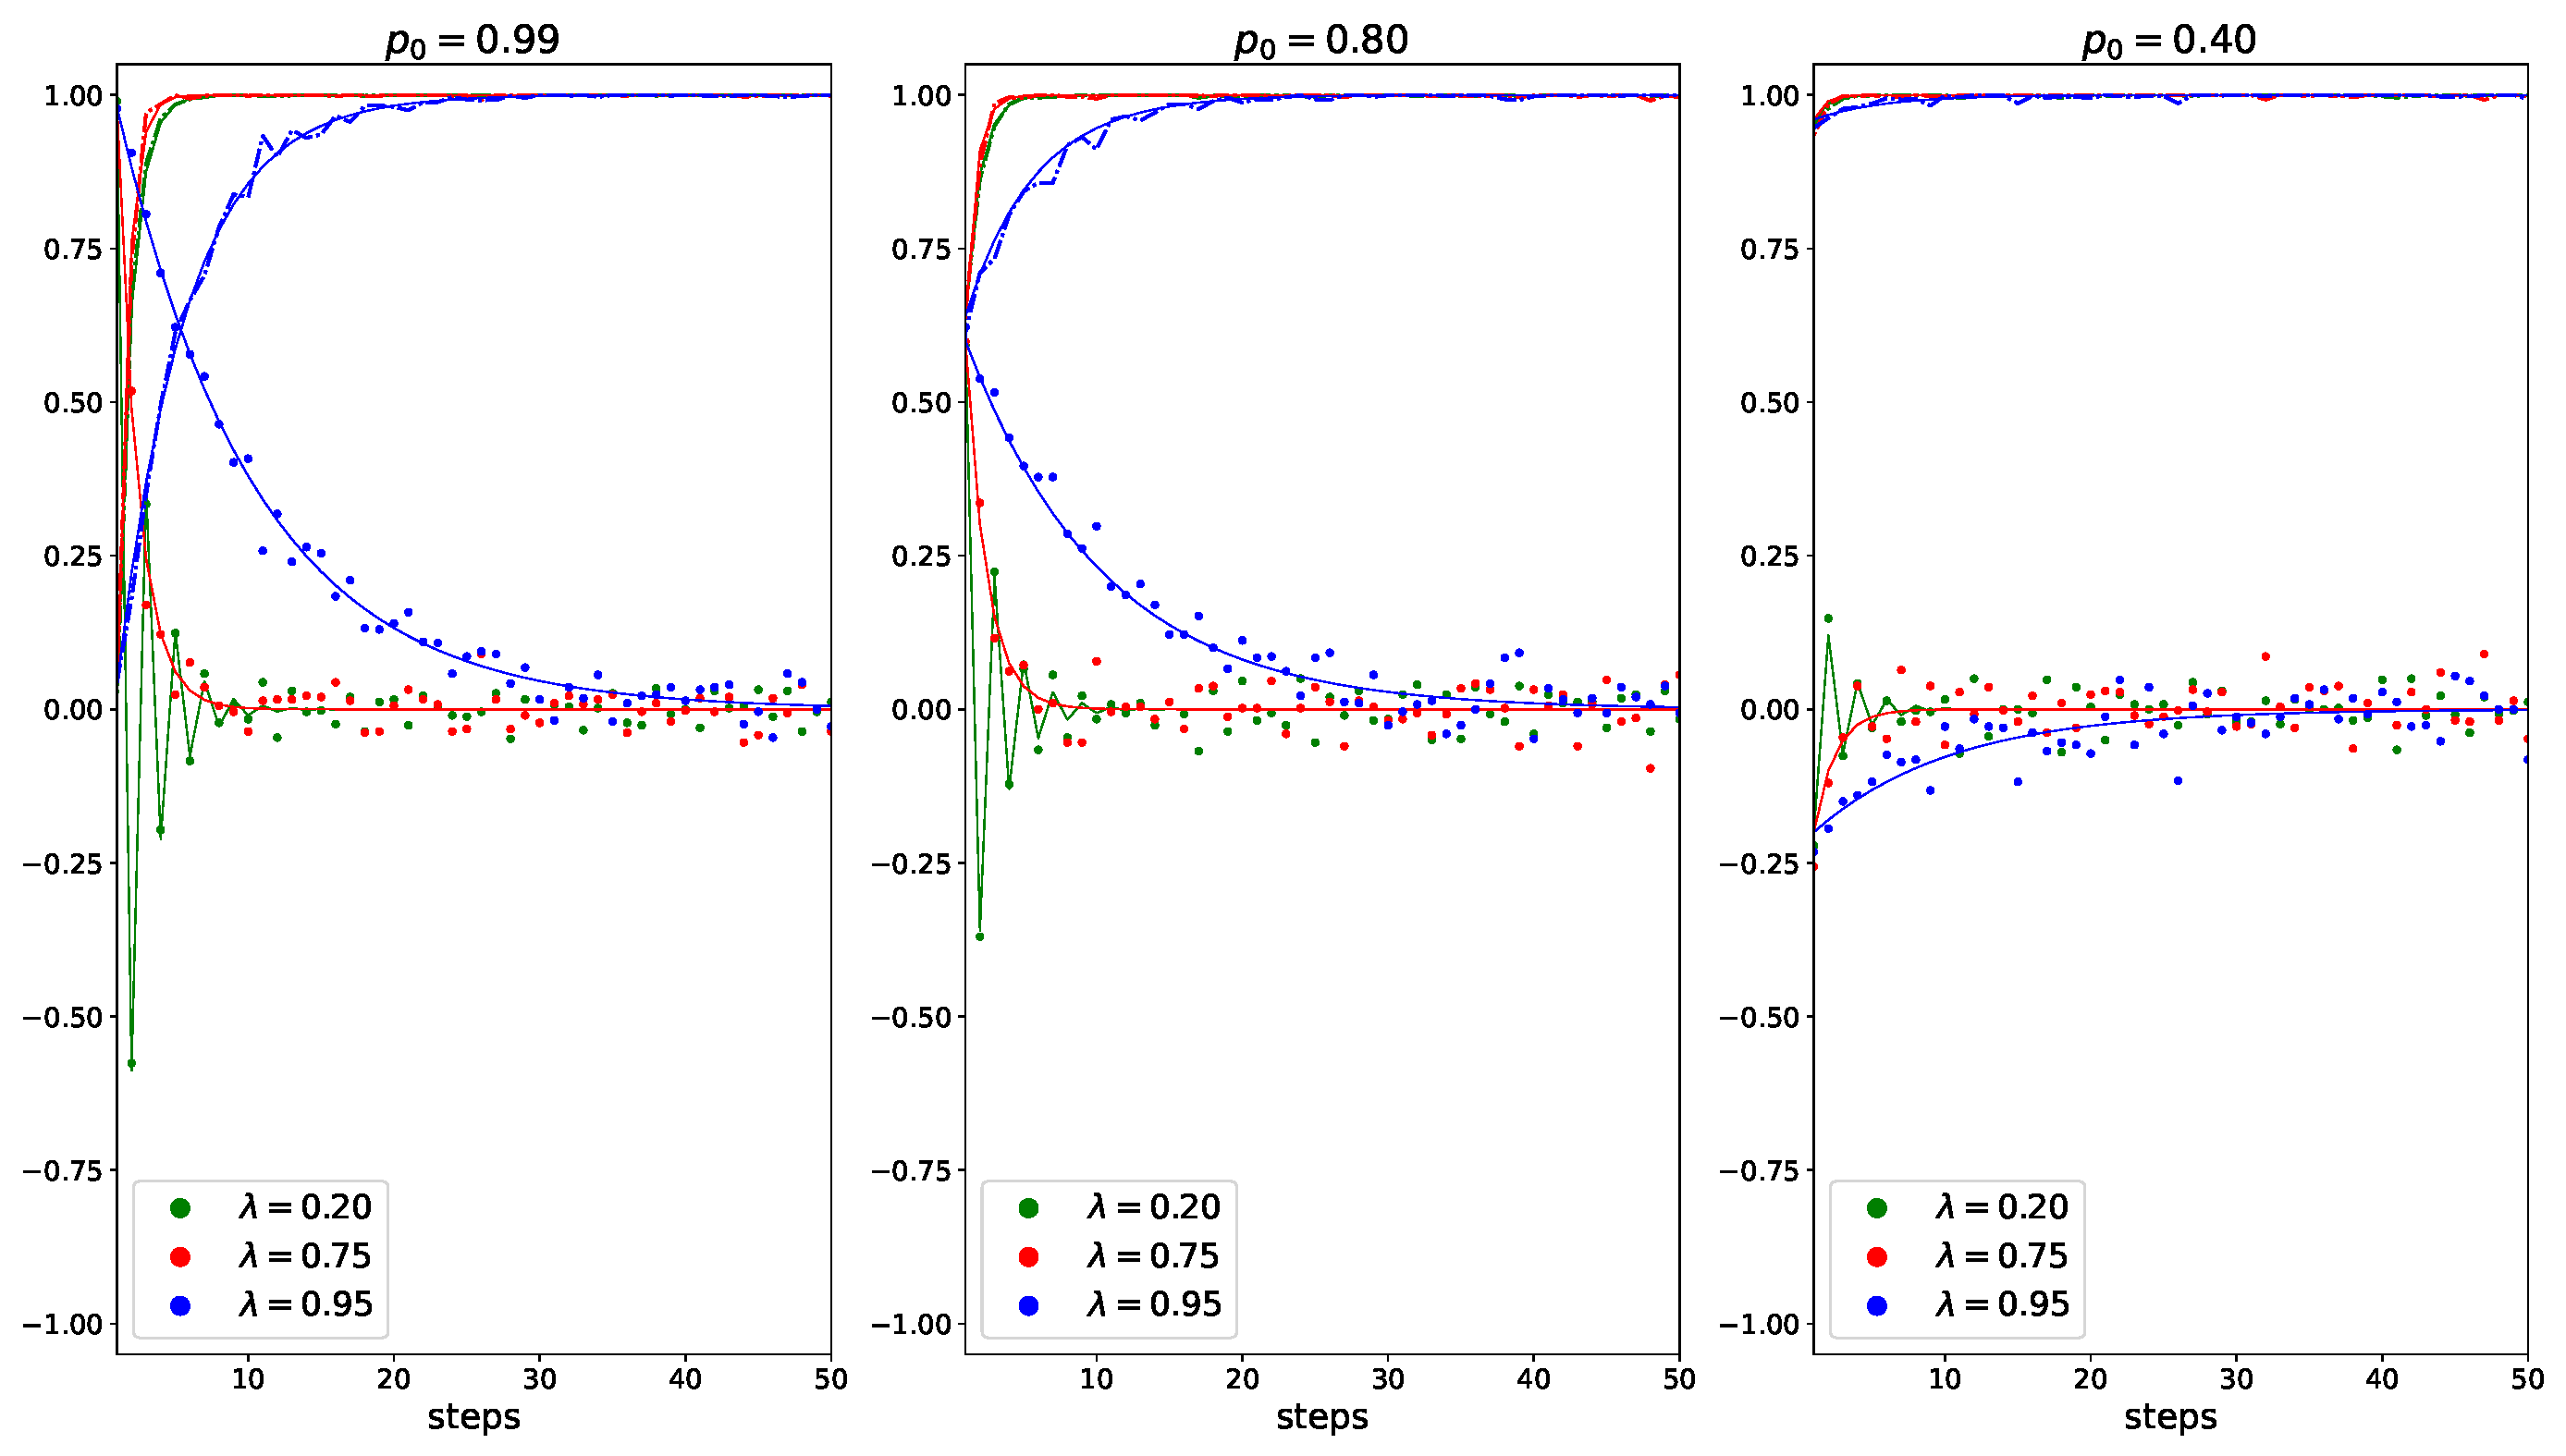
\includegraphics[width=1\textwidth]{../../simulations/e_step_1000_walks_50_steps_type_success_punished}
    \end{frame}

    \begin{frame}{Walk probabilities properties}
        \begin{flalign*}
            EP_{t} & =(2\lambda-1)^{t}p_{0}+\frac{1-(2\lambda-1)^{t}}{2} &
        \end{flalign*}
        \vspace{-5mm}
        \begin{flalign*}
            \lim_{t\to+\infty}EP_{t} & =\frac{1}{2} &
        \end{flalign*}
        \onslide<2->
        \begin{flalign*}
            Var\,P_{t} & =(3\lambda^{2}-2\lambda)^{t}p_{0}^{2}+\sum_{i=0}^{t-1}K(i;p_{0},\lambda)(3\lambda^{2}-2\lambda)^{t-1-i}-k(t;p_{o},\lambda)^{2} &
        \end{flalign*}
        \vspace{-5mm}
        \begin{flalign*}
            \lim_{t\to+\infty}Var\,P_{t} & =\frac{\frac{1}{2}(1-\lambda^{2})}{-3\lambda^{2}+2\lambda+1}-\frac{1}{4} &
        \end{flalign*}
    \end{frame}

    \begin{frame}{Example - RW probabilities}
        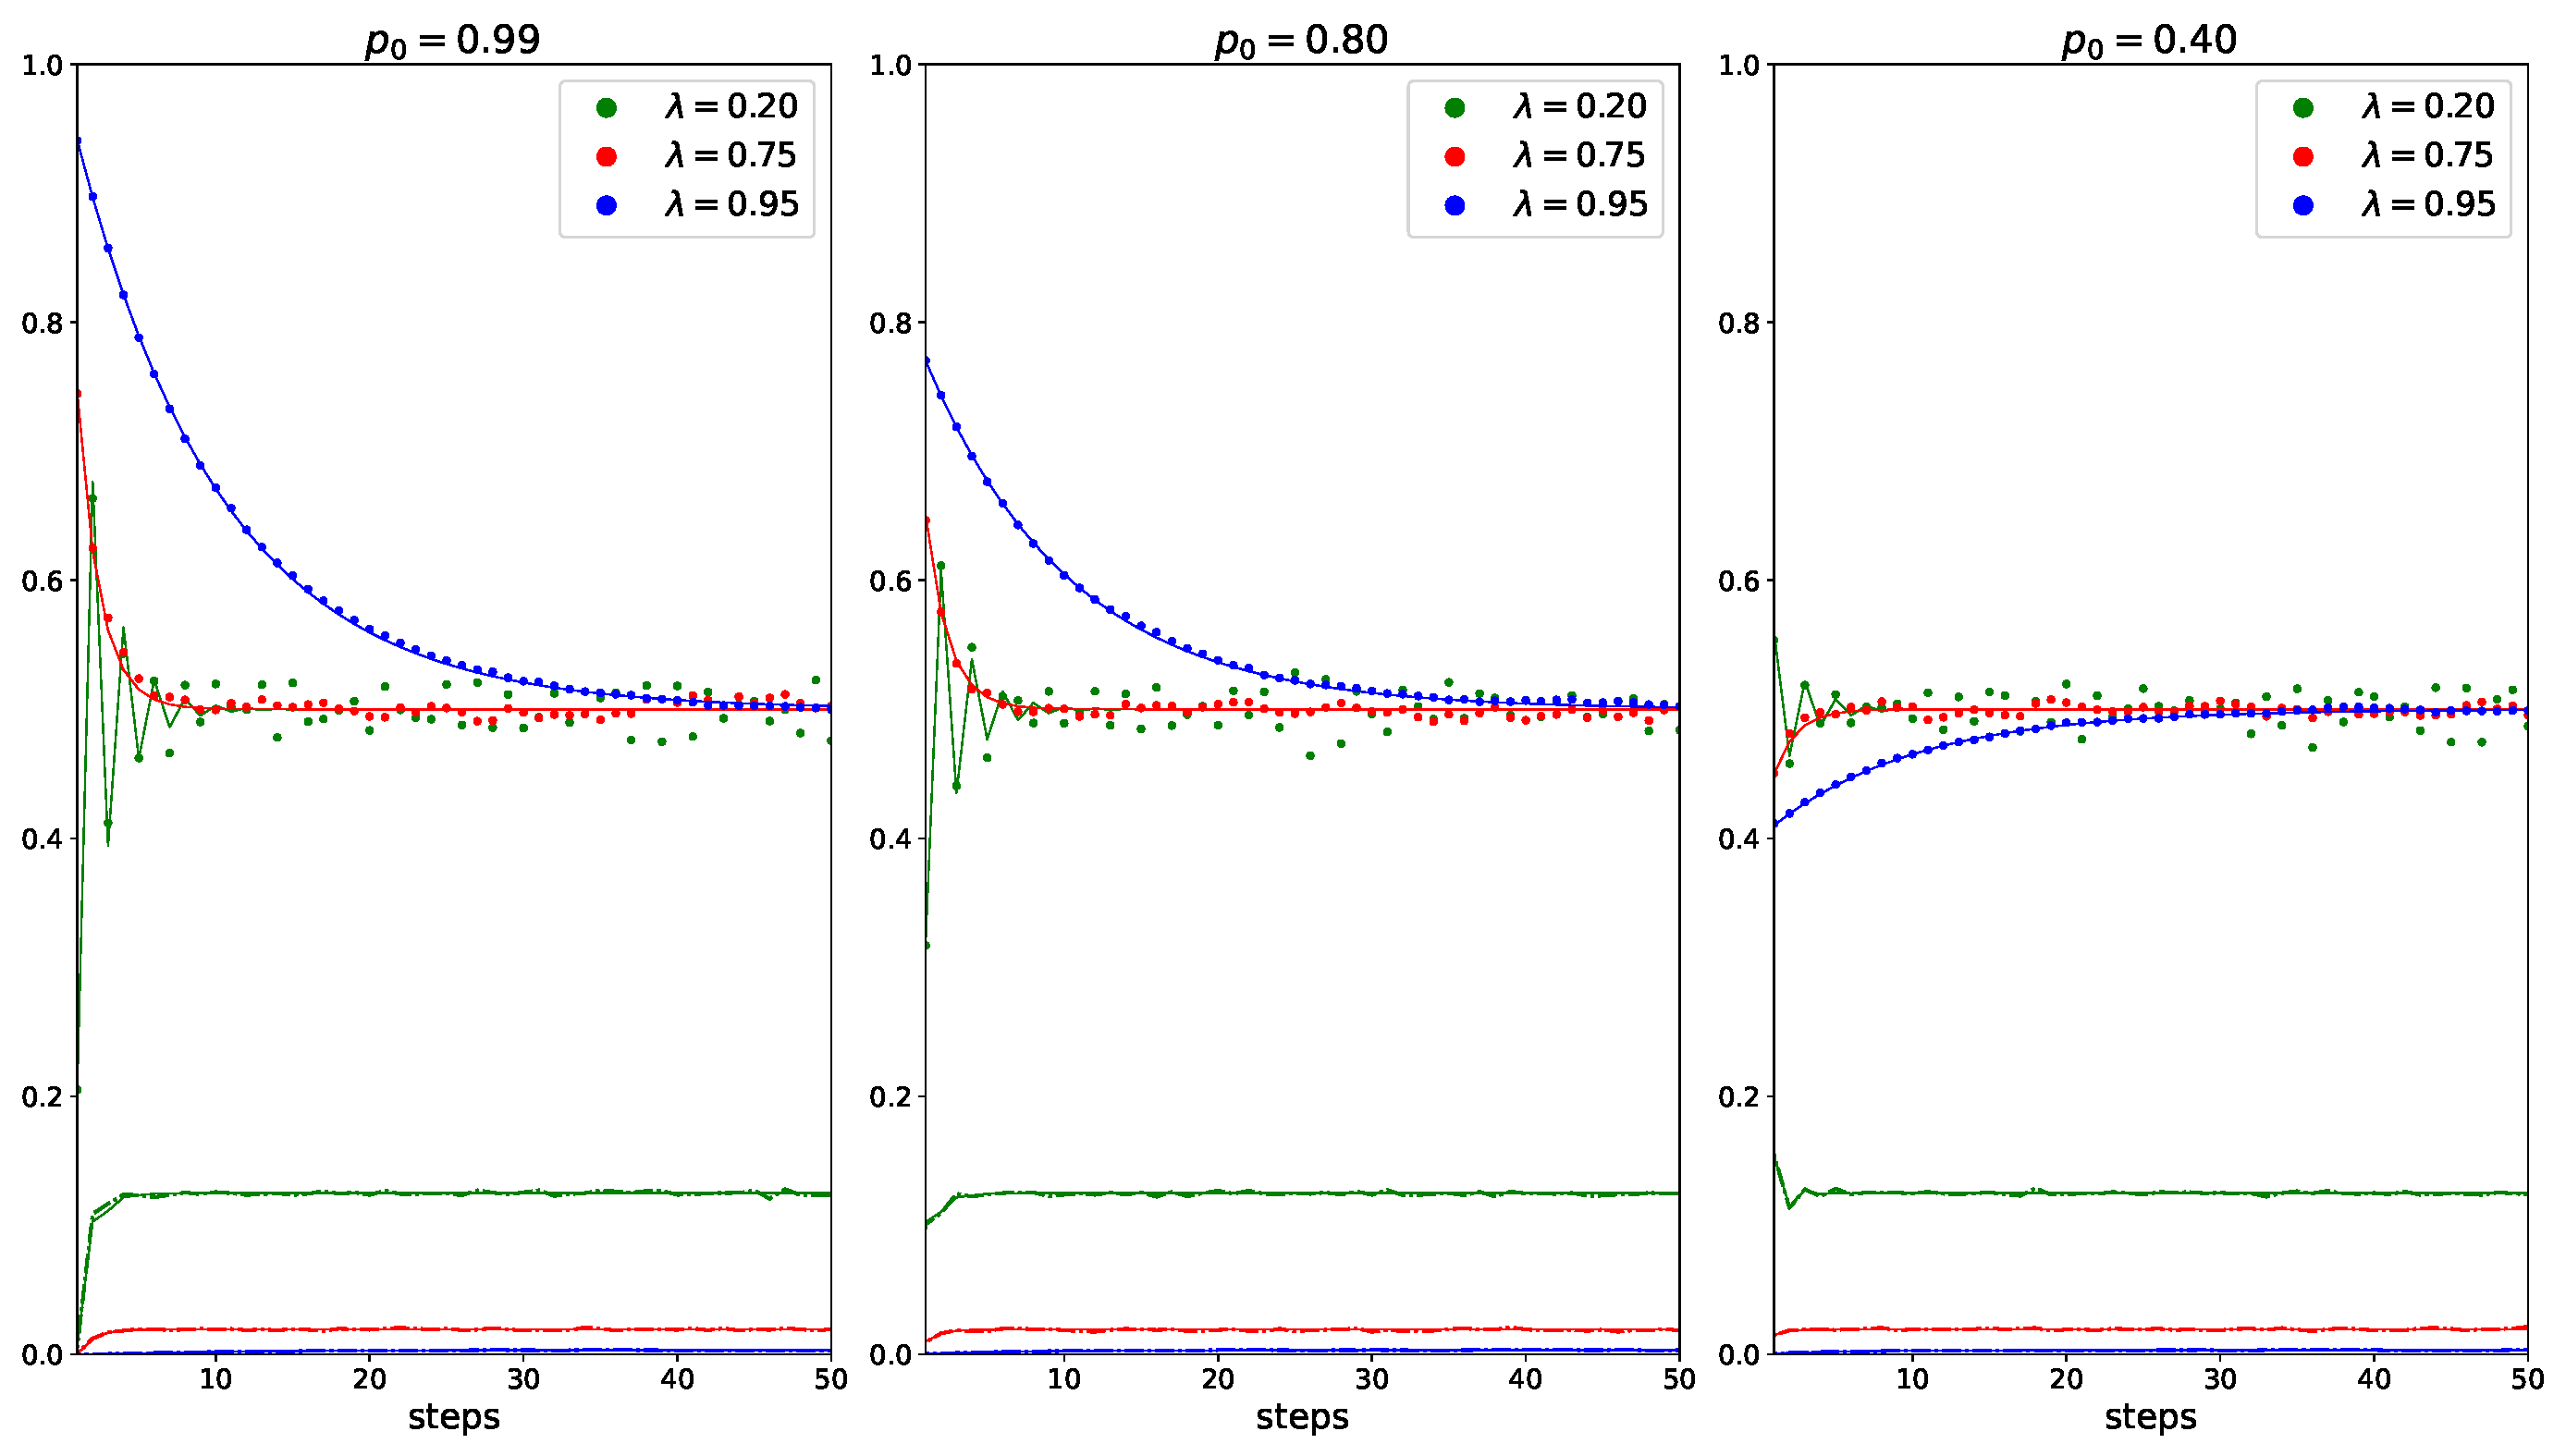
\includegraphics[width=1\textwidth]{../../simulations/e_probability_1000_walks_50_steps_type_success_punished}
    \end{frame}

    \begin{frame}{Walk position properties}
        \begin{flalign*}
            ES_{t} & =S_{0}+(2p_{0}-1)\frac{1-(2\lambda-1)^{t}}{2(1-\lambda)} &
        \end{flalign*}
        \vspace{-5mm}
        \begin{flalign*}
            \lim_{t\to+\infty}ES_{t} & =S_{0}+\frac{(2p_{0}-1)}{2(1-\lambda)} &
        \end{flalign*}
        \onslide<2->
        \begin{flalign*}
            Var\,S_{t} & =t+4\sum_{i=0}^{t-1}\sigma(i;p_{0},0,\lambda)-a(t;p_{0},\lambda) &
        \end{flalign*}
        \vspace{-5mm}
        \begin{flalign*}
            \lim_{t\to+\infty}Var\,S_{t} & =c_{1}(p_{0},\lambda)t+c_{2}(p_{0},\lambda) &
        \end{flalign*}
    \end{frame}

    \begin{frame}{Example - RW position}
        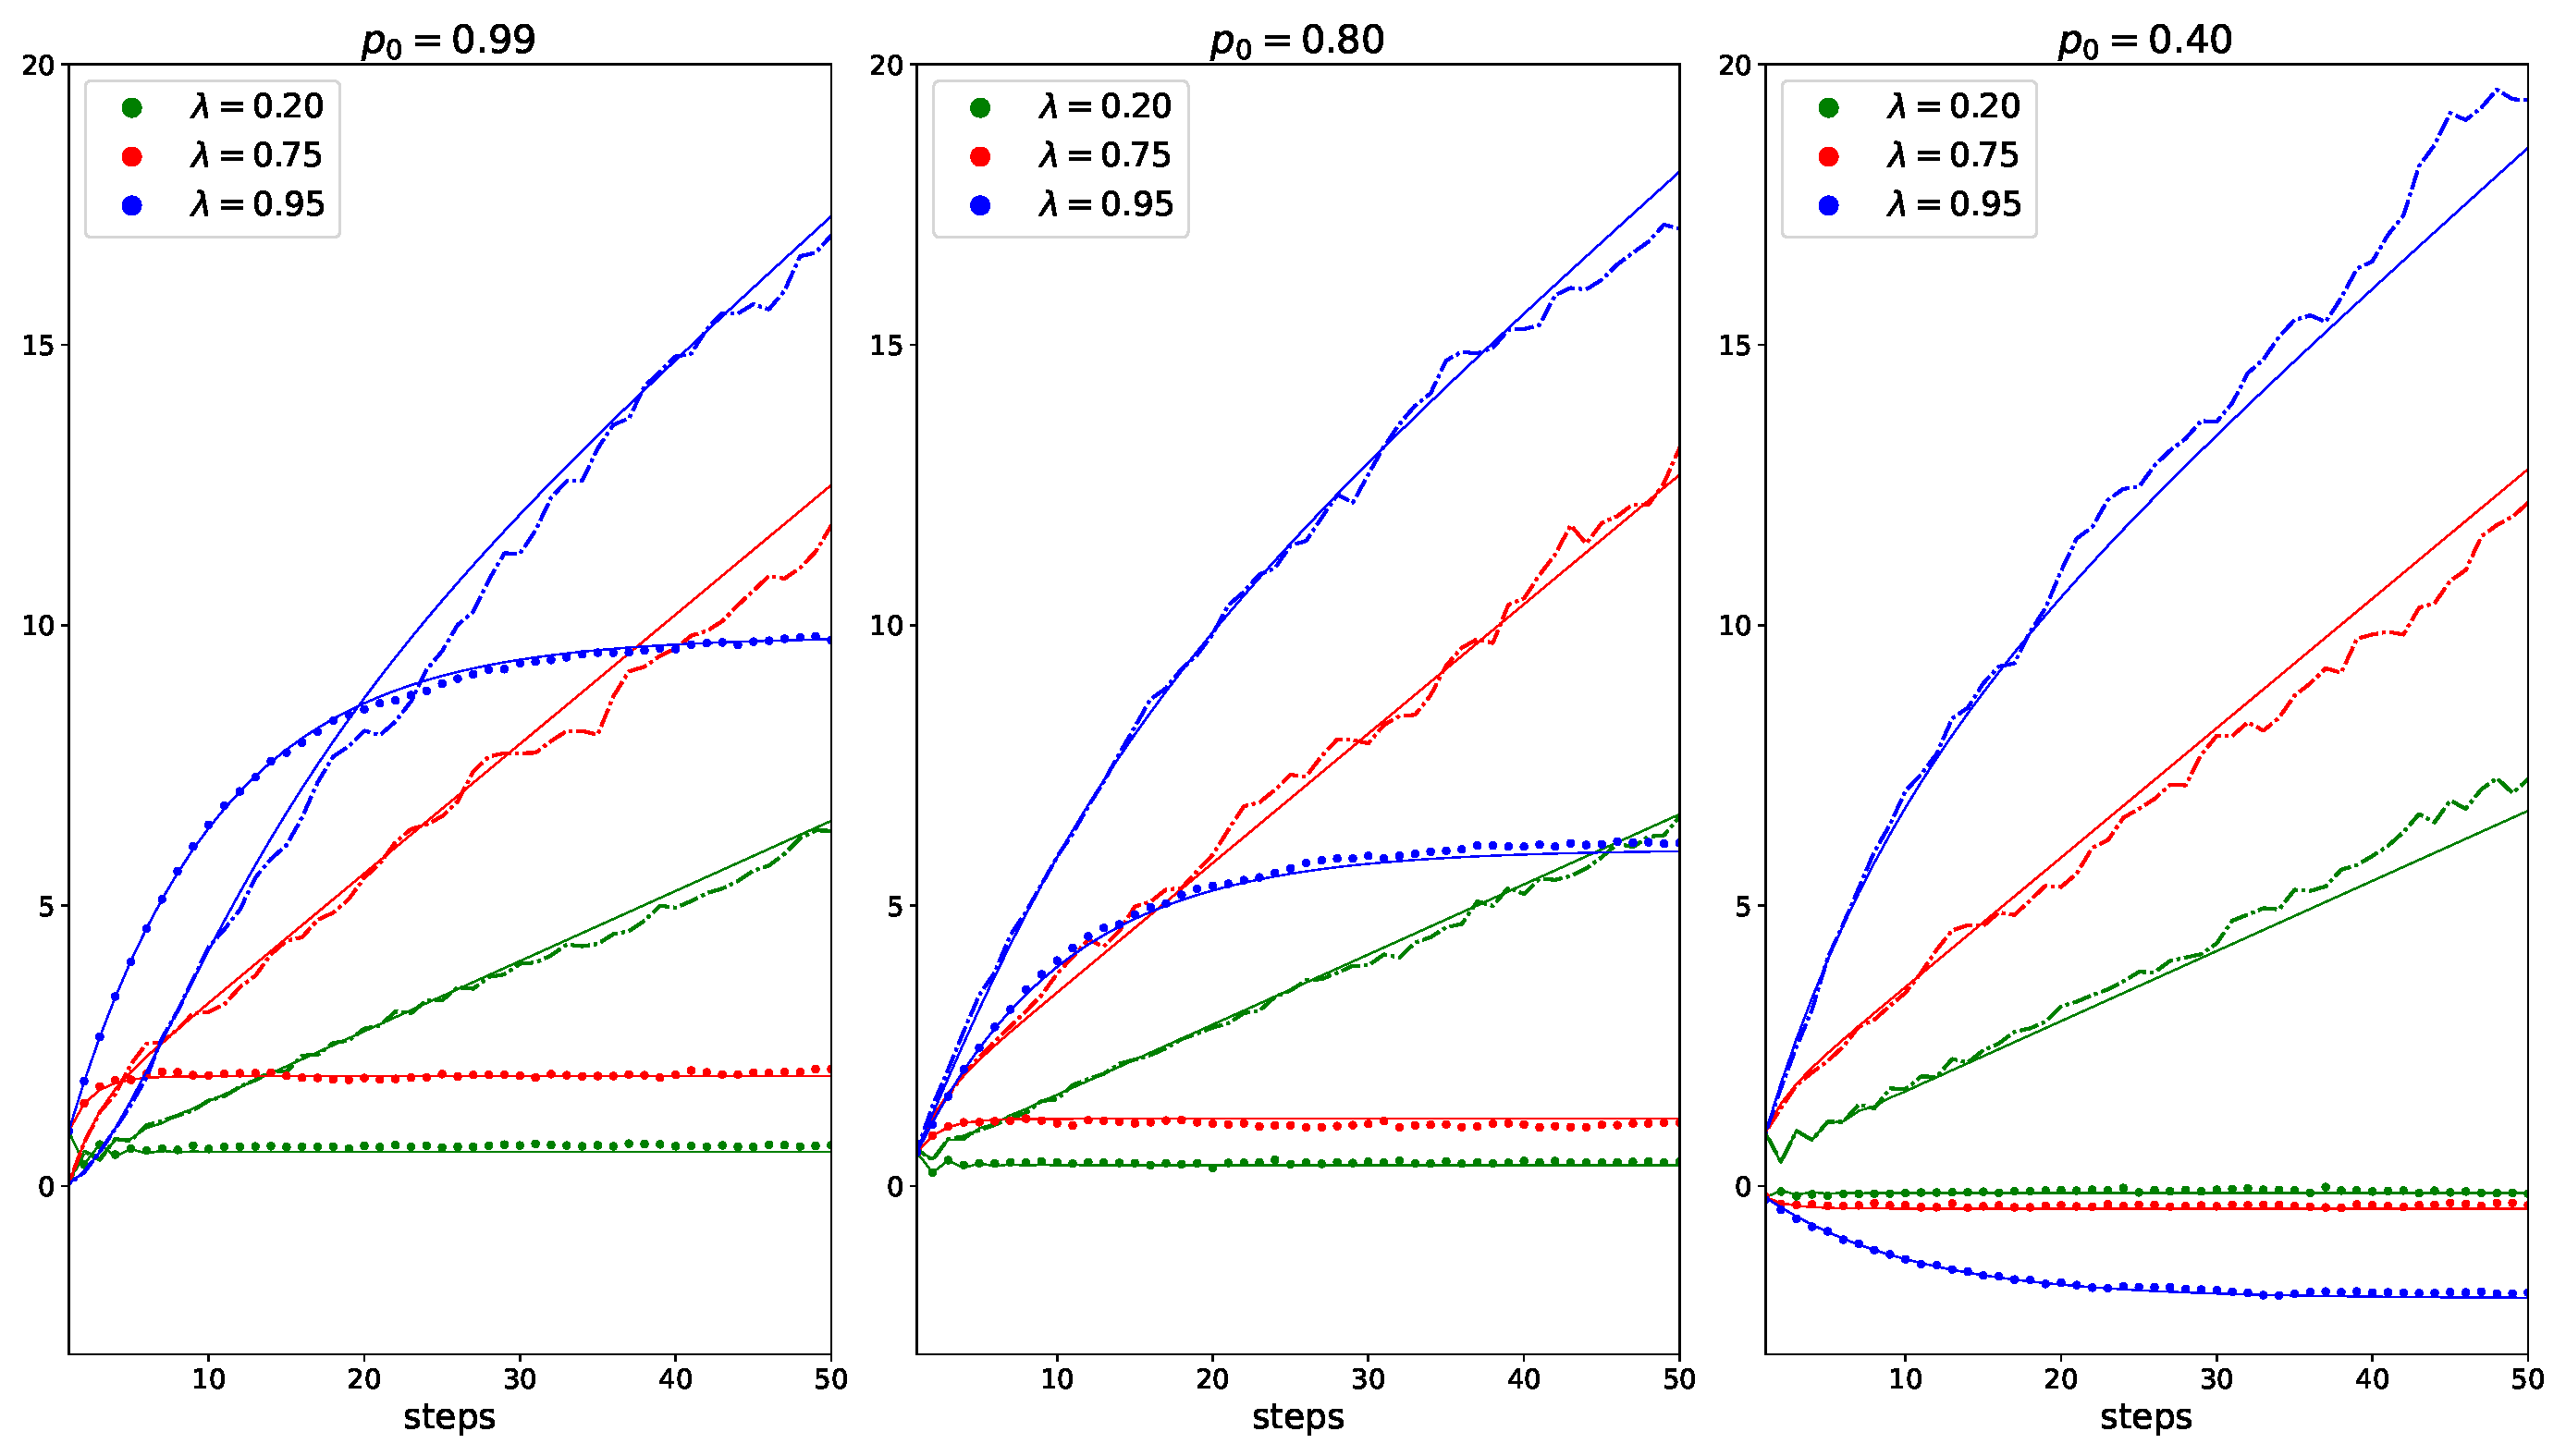
\includegraphics[width=1\textwidth]{../../simulations/e_position_1000_walks_50_steps_type_success_punished}
    \end{frame}

    \begin{frame}{Success rewarding model}
        \begin{flalign*}
            EX_{t} & =2p_{0}-1 &
        \end{flalign*}
        \vspace{-8mm}
        \begin{flalign*}
            Var\,X_{t} & =4p_{0}(1-p_{0}) &
        \end{flalign*}
        \begin{flalign*}
            EP_{t} & =p_{0} &
        \end{flalign*}
        \vspace{-8mm}
        \begin{flalign*}
            Var\,P_{t} & =(2\lambda-\lambda^{2})^{t}p_{0}^{2}+p_{0}(1-\lambda)^{2}\sum_{i=0}^{t-1}(2\lambda-\lambda^{2})^{i}-p_{0}^{2} &
        \end{flalign*}
        \begin{flalign*}
            ES_{t} & =S_{0}+t(2p_{0}-1) &
        \end{flalign*}
        \vspace{-8mm}
        \begin{flalign*}
            Var\,S_{t} & =4p_{0}(1-p_{0})t^{2}+a(p_{0},\lambda)t-a(p_{0},\lambda)\frac{1-(2\lambda-\lambda^{2})^{t}}{(1-\lambda)^{2}} &
        \end{flalign*}
    \end{frame}

    \begin{frame}{Two-parameter model}
        \begin{itemize}
            \item Two $\lambda$ parameters each affecting one direction of the walk
            \item Again two variants -- success punishing and success rewarding
            \onslide<2->\begin{flalign*}
                            X_{t-1} & =1\rightarrow p_{t}=\lambda_{0} p_{t-1} &
                            X_{t-1} & =-1\rightarrow p_{t}=1-\lambda_{1}(1-p_{t-1}) &
            \end{flalign*}
            \vspace{-5mm}
            \begin{itemize}
                \item[-->]<2-> ``Two-parameter success punishing model''
            \end{itemize}
            \onslide<3->\begin{flalign*}
                            X_{t-1}&=1\rightarrow p_{t}=1-\lambda_{0}(1-p_{t-1})&
                            X_{t-1}&=-1\rightarrow p_{t}=\lambda_{1} p_{t-1}&
            \end{flalign*}
            \vspace{-5mm}
            \begin{itemize}
                \item[-->]<3-> ``Two-parameter success rewarding model''
            \end{itemize}
        \end{itemize}
    \end{frame}

    \begin{frame}{Example - two-parameter success punishing model}
        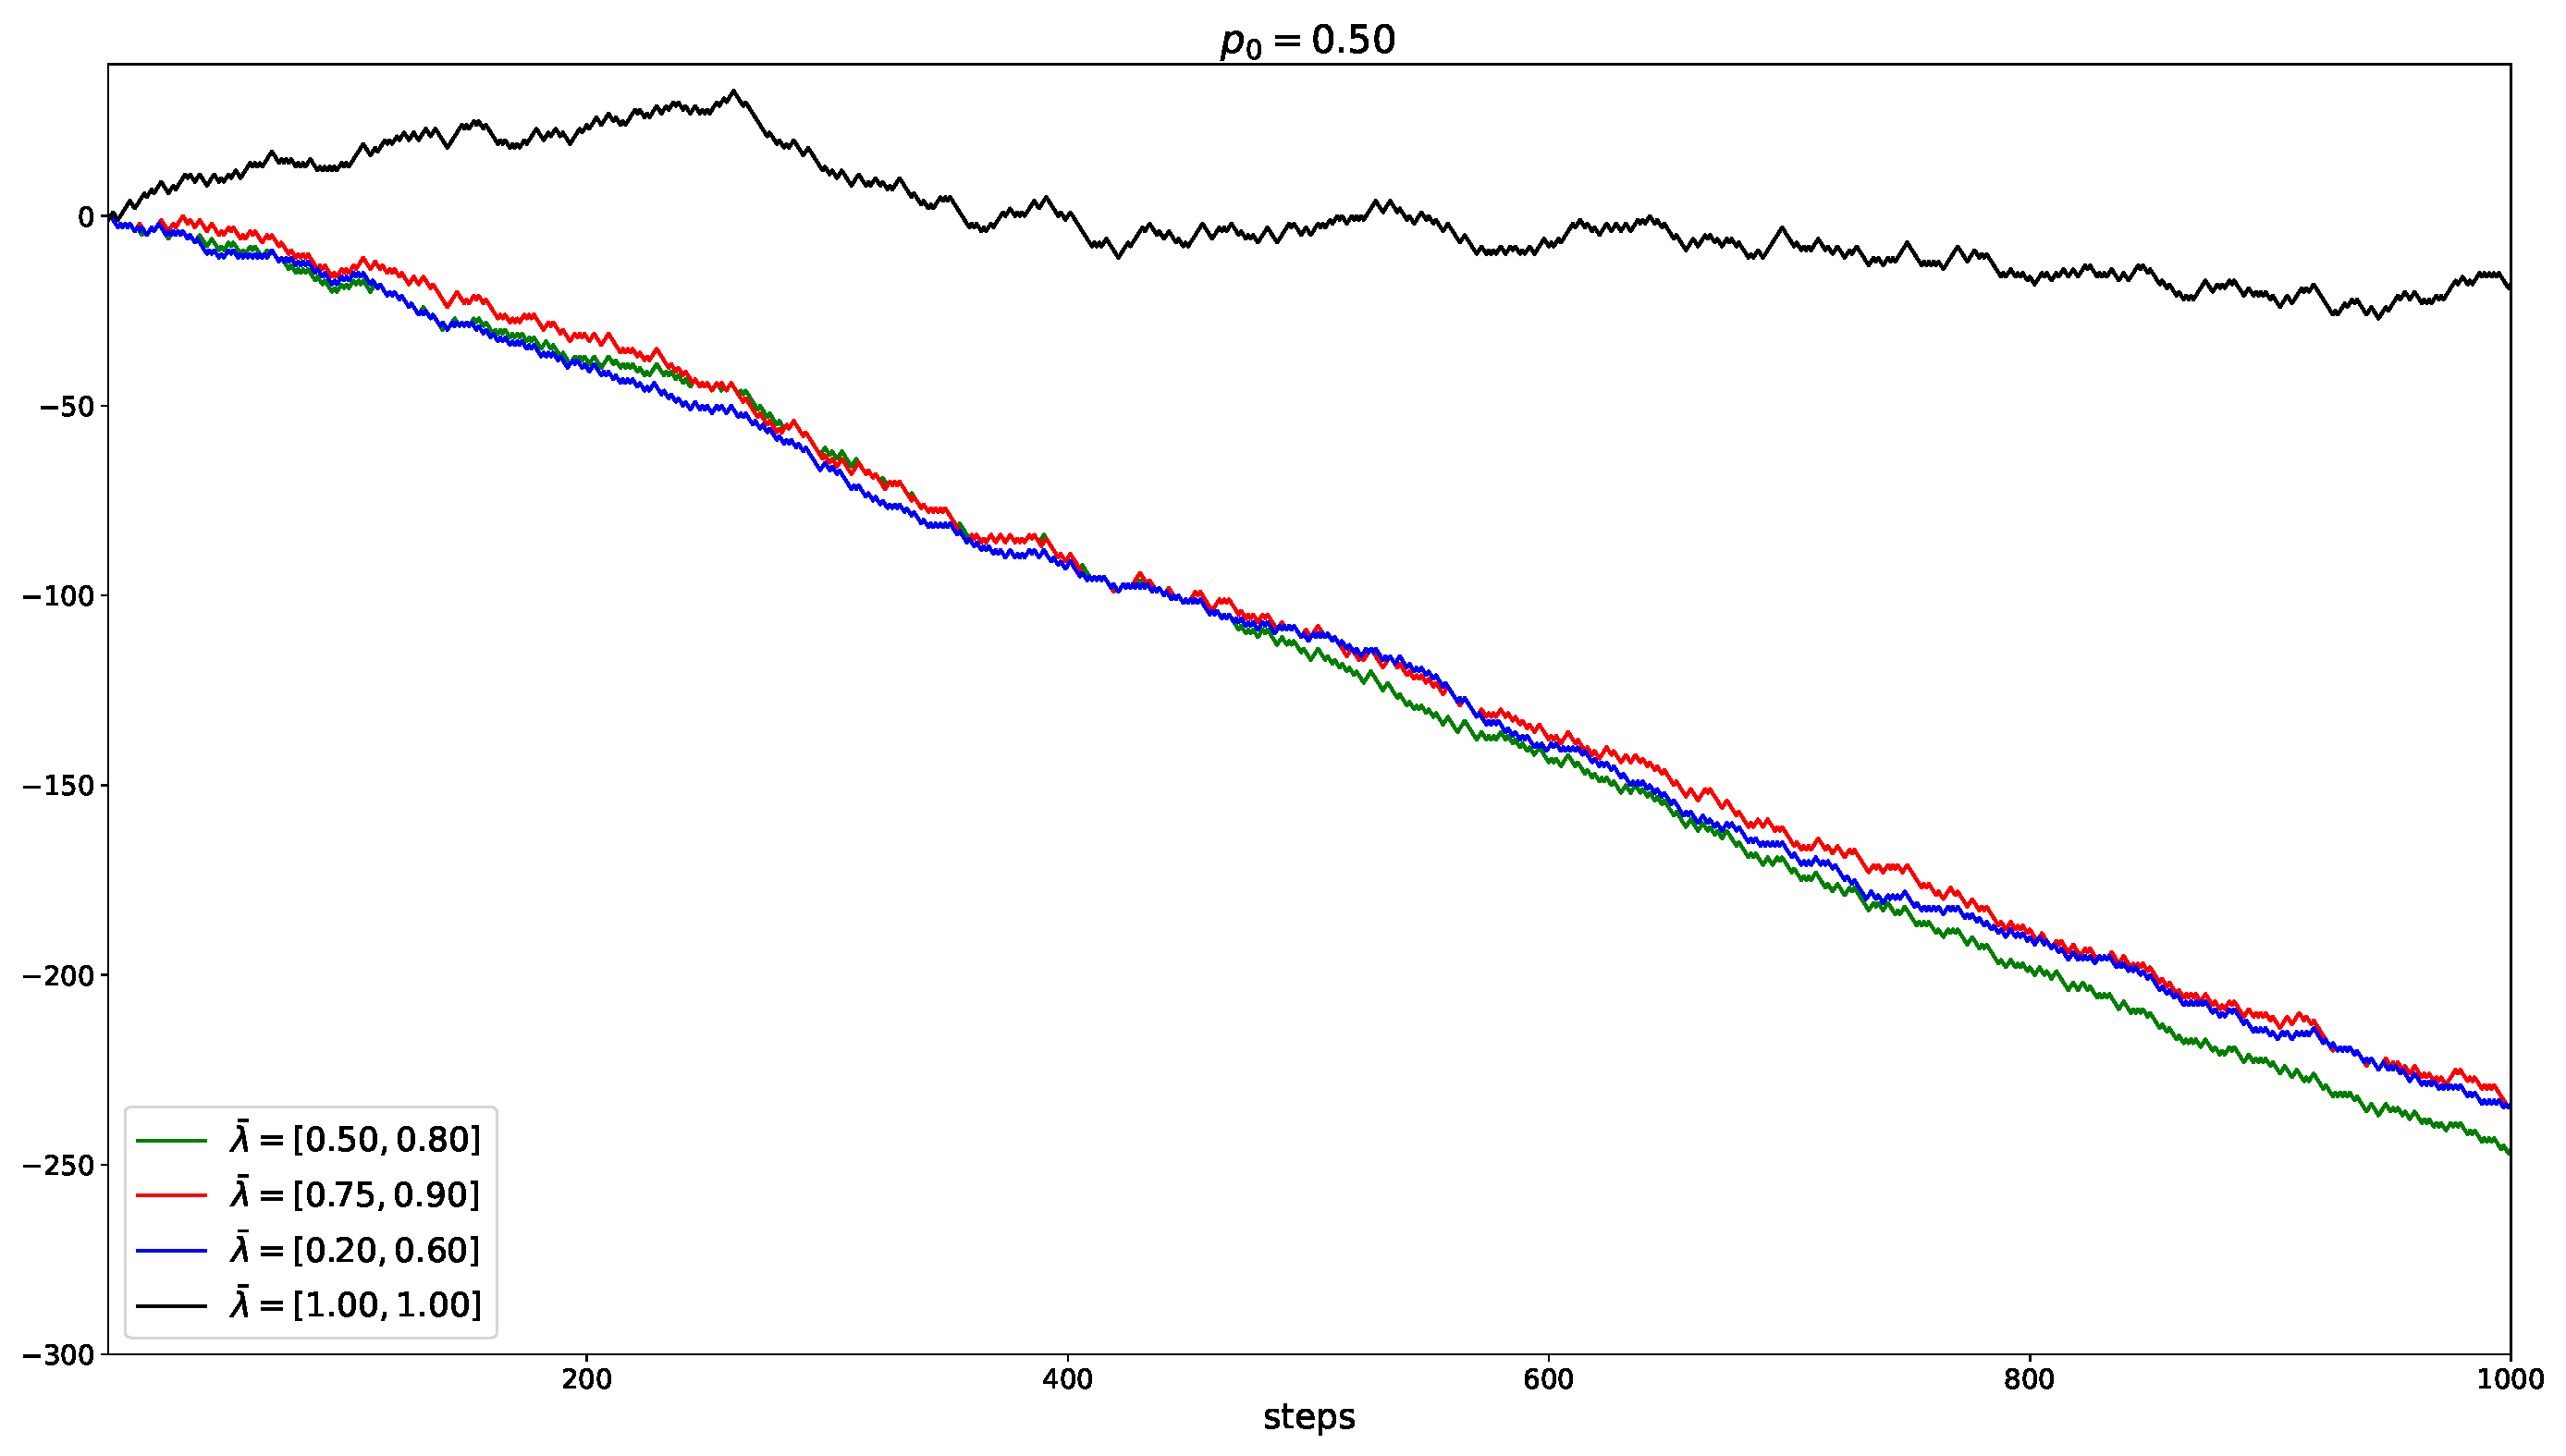
\includegraphics[width=1\textwidth]{../../simulations/single_walk_1000_steps_type_success_punished_two_lambdas}
    \end{frame}

    \begin{frame}{Model fitting}
        \begin{enumerate}
            \item Find $\overrightarrow{\lambda}$ with known $p_{0}$, model type
            \item Find $p_{0}$ with known $\overrightarrow{\lambda}$, model type
            \item Find $p_{0},\,\overrightarrow{\lambda}$ with known model type
            \item Find model type without any prior knowledge
        \end{enumerate}
    \end{frame}

    \begin{frame}{Model fitting}
        \begin{enumerate}
            \item Find $\overrightarrow{\lambda}$ with known $p_{0}$, model type
            \item Find $p_{0}$ with known $\overrightarrow{\lambda}$, model type
            \item Find $p_{0},\,\overrightarrow{\lambda}$ with known model type
            \begin{itemize}
                \item Using maximal likelihood estimate \& numerical optimization
            \end{itemize}
            \item Find model type without any prior knowledge
        \end{enumerate}
    \end{frame}

    \begin{frame}{Model fitting}
        \begin{enumerate}
            \item Find $\overrightarrow{\lambda}$ with known $p_{0}$, model type
            \item Find $p_{0}$ with known $\overrightarrow{\lambda}$, model type
            \item Find $p_{0},\,\overrightarrow{\lambda}$ with known model type
            \begin{itemize}
                \item Using maximal likelihood estimate \& numerical optimization
            \end{itemize}
            \item Find model type without any prior knowledge
            \begin{itemize}
                \item Using Akaike information criterion \& numerical optimization
            \end{itemize}
        \end{enumerate}
    \end{frame}

    \begin{frame}{Real life application}
        \begin{itemize}
            \item Success rewarding model well suited for modelling tennis matches
            \item Model trained on 2009--2018 men Grand Slam tournaments
            \item<2-> Model applied on 2019 US Open
            \begin{itemize}
                \item<2-> Live betting against bookmaker
                \item<2-> $0.52$ units total necessary bankroll
                \item<2-> $2.24$ units total profit $\rightarrow$ $430\%$ ROI
                \item<3-> Only 128 bets placed
            \end{itemize}
        \end{itemize}
    \end{frame}

    \begin{frame}{Summary}
        \begin{itemize}
            \item A specific model of a random walk with memory
            \item Model properties derived
            \item Application shows big future potential of the model
            \item Possible applications in a set of real life scenarios
        \end{itemize}
    \end{frame}

    \begin{frame}[plain]
        \begin{quote}
            \begin{center}
                \huge{Thank you.}
            \end{center}
            \vspace{10mm}
            \begin{center}
                \large{tom@skourim.com}
            \end{center}
        \end{quote}
    \end{frame}

\end{document}
